\chapter{Gain in function of the frequency}
In a real op-amp the open loop gain ($A_{ol}$) is a function of the input frequency. In this experience we explored systematically this behaviour using 2 different circuits, one for the lower frequencies and the other for the higher one. After this study we built a non inverting amplifier with $\approx 10$ and $\approx 100$ gain for measuring its bandwidth.

\section{Materials}
\begin{itemize}
\item Operational amplifier uA741
\item Resistors, trimmer
\item Power supply RIGOL DP831A
\item Waveform generator RIGOL DG1032
\item Multimeter RIGOL DM3068
\item Oscilloscope RIGOL MS02102A
\end{itemize}
The resistor chosen were $R_1, R_2, R_3 = 10\text{k} \Omega$, $R_4 = 10 \Omega$, $R_5 = 100 \Omega, R_6 = 1\text{k}\Omega$ with an error of $5\%$ of the value.
\section{Experimental setup}
\begin{figure}[H]
\centering
\begin{minipage}{.5\textwidth}
  \centering
\begin{circuitikz}
\draw(0,0) node[op amp] (opamp) {}
	%(opamp.+) node[left] {$v_+$}
	(opamp.+) to[short] (-1.5,-.49)to[short](-1.5,-1.5)to[short](-2.5,-1.5)
	(opamp.out) to [short,-o](1.8,0) node[right] {$v_o$}
	(opamp.down) ++(0,-.5) node[below] {$-v_{cc}$} -- (opamp.down)
	(opamp.up) ++ (0,.5) node[above] {$+v_{cc}$} -- (opamp.up)
	(opamp.down) ++ (0,-.25)to[C,/tikz/circuitikz/bipoles/length=1cm] (1,-.8)node[ground,rotate = 90,yshift = 1em] {}
	(opamp.up) ++ (0,.25)to[C,/tikz/circuitikz/bipoles/length=1cm] (1,.8)node[ground,rotate = 90,yshift = 1em] {};
	\draw(opamp.-) to[short](-2.5,.49) to[R=$R_3$,-*](-2.5,2.2)node[above]{$v_a$} to[R,l=$R_2$](1.5,2.2) to[short](1.5,0);
	\draw(-2.5,.49)to[R,l_=$R_4$](-2.5,-1.5) node[ground]{};
	\draw(-4.5,.49)node[ground]{}to[sV](-4.5,2.2) to[R = $R_1$](-2.5,2.2);
\end{circuitikz}
\caption{$A_{ol}$ measure low frequencies}
\end{minipage}%
\begin{minipage}{.5\textwidth}
\begin{circuitikz}
\draw(0,0) node[op amp] (opamp) {}
	%(opamp.+) node[left] {$v_+$}
	(opamp.+) ++ (-.3,0) node[ground] {} -- (opamp.+) 
	(opamp.out) to [short,-o](1.8,0) node[right] {$v_o$}
	(opamp.down) ++(0,-.5) node[below] {$-v_{cc}$} -- (opamp.down)
	(opamp.up) ++ (0,.5) node[above] {$+v_{cc}$} -- (opamp.up)
	(opamp.down) ++ (0,-.25)to[C,/tikz/circuitikz/bipoles/length=1cm] (1,-.8)node[ground,rotate = 90,yshift = 1em] {}
	(opamp.up) ++ (0,.25)to[C,/tikz/circuitikz/bipoles/length=1cm] (1,.8)node[ground,rotate = 90,yshift = 1em] {};
	\draw(opamp.-) to[short](-2.5,.49) to[short,-*](-2.5,2.2)node[above]{$v_a$} to[R,l=$R_2$](1.5,2.2) to[short](1.5,0);
	\draw(-4.5,.49)node[ground]{}to[sV](-4.5,2.2) to[R,l=$R_1$](-2.5,2.2);
\end{circuitikz}
\caption{$A_{ol}$ measure high frequencies}
\end{minipage}
\end{figure}
In this experience we took the measurament in all circuis by changing the frequency of the input, that was a  sine wave signal 1 V peak-peak. The voltage chosen is not important, because we are interested in the ratio between the amplitude of two signal.
In the first circuit was used for calculating the gain in the open loop configuration $A_{ol}$ in low frequencies by measuring $v_a$ and $v_{o}$. This circuit was chosen for low freqencies instead of the second one, beacause the gain is too high for allowing us to acquiring directly the voltage difference between the two input pins. 
We didn't measure at lower frequencies than 30 Hz because the noise didn't allow us to make a reliable extimate of the amplitude of the two signals.\\
In the second circuit we measured $v_{o}$ and the voltage of the non inverting pin $v_a$. The frequencies measured went from 10 - 200 kHz, because with high frequencies the absulute value of $A_{ol}$ is low enough.\\
In the last two circuits we built an non inverting amplifier with gain of 100 and 10.
\begin{figure}[H]
  \centering
  \begin{circuitikz}
 \draw(0,0) node[op amp,yscale=-1] (opamp) {}
%(opamp.+) node[left] {$v_+$}
(opamp.-) ++ (-.3,0) -- (opamp.-) 
(opamp.-) ++ (-.3,0) to[R,l_=$R_4-R_5$] (-3,-0.5) to (-3,-1) node[ground]{}
(opamp.-) ++ (-.3,0) -- (-1.5,-1.8) to[R,l_=$R_6$] (1,-1.8) -- (1,0)
(opamp.out) node[right] {$v_o$}
(opamp.up) ++(0,-.5) node[below] {$-v_{cc}$} -- (opamp.up)
(opamp.down) ++ (0,.5) node[above] {$+v_{cc}$} -- (opamp.down);
\draw(-4,-1) to[sV,l=$v_{in}$] (-4,.5) to[short] (opamp.+);
\draw(-4,-1) node[ground] {};
\end{circuitikz}
\caption{Non inverting amplifier}
\end{figure}
\section{Data Analysis}
<<<<<<< HEAD

In the first circuit we can extimate the open loop gain by using $A_{ol} = - \frac{v_{o}}{v_A} \frac{R_3 + R_4}{R_4}$.
In the second circuit we calculated $A_{ol} = - \frac{v_{o}}{v_-}$. \\
We can see from the plot that the data appears to be on a straight line, we can also see if that line is compatible with the values in the datasheet. We can compute the theoretical open loop gain with: $$A_{ol}^{teo}(f) = \frac{A}{1 + j\frac{f}{f_0}}$$ Where $A = 1.5 \times 10^5$ and $f_0 = 8$ Hz are two parameters available in the datasheet, $j$ is the immaginary unit and $f$ is the frequency. We can see from the plot that our data is consistent with the theory and the datasheet.
For the last two circuit we plotted $H = \frac{v_{o}}{v_-}$. We can see if the data is in accordance with the theory by computing $\frac{\frac{A}{1 + A\beta}}{1 + j \frac{f}{(1 + A\beta)f_0}}$
=======
\begin{figure}[H]
\centering
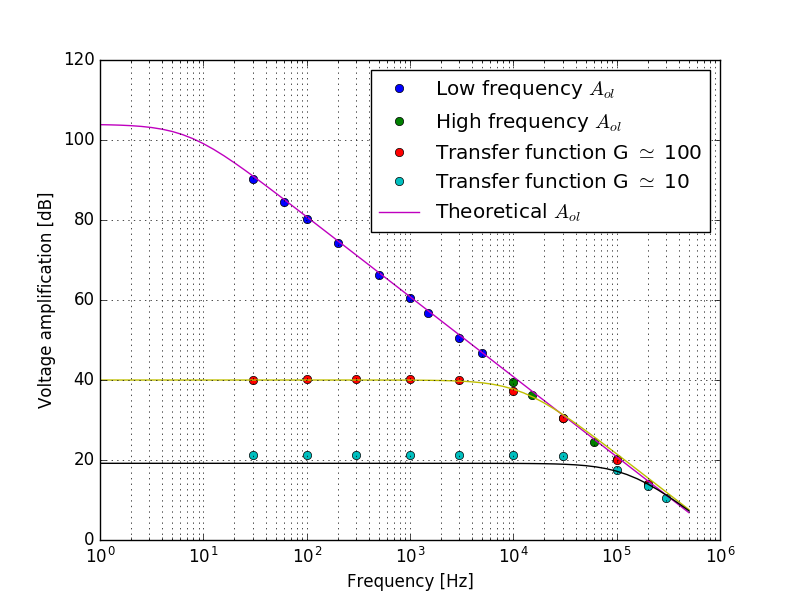
\includegraphics[width=.7\textwidth]{4/decibel.png}
\end{figure}
In the first circuit we can extimate the open loop gain by using $A_{ol} = - \frac{v_{o}}{v_a} \frac{R_3 + R_4}{R_4}$.
In the second circuit we calculated $A_{ol} = - \frac{v_{o}}{v_a}$. \\
We can see from the plot that the data appears to be on a straight line, we can also see if that line is compatible with the values in the datasheet. We can compute the theoretical open loop gain with: $$A_{ol}^{teo}(f) = \frac{A}{1 + j\frac{f}{f_0}}$$ Where $f_0 = 8$ Hz is a parameters available in the datasheet and  $A = 1.5 \times 10^5$ was obtained with the best fit, $j$ is the immaginary unit and $f$ is the frequency. We can see from the plot that our data is consistent with the theory and the datasheet.\\
For the last two circuit we plotted $H = \frac{v_{o}}{v_{in}}$, the theoretical curve is the following:
\[H(f) = \frac{\frac{A_{ol} }{1 + A_{ol} \beta}}{1 + j \frac{f}{(1 + A_{ol} \beta)f_0}}\]
>>>>>>> b85e6bac9be578443450962c623a96d1c11a0c18
